\documentclass[10pt]{article}  

%%%%%%%% Preamble %%%%%%%%%%%%
\title{Degree work}
\usepackage{listings}
\usepackage[utf8]{inputenc} % File coding uses utf8
\usepackage{amsmath} % Extra commands for math
\usepackage{amsthm}
\usepackage{amssymb} % Math symbols 
\newtheorem{definition}{Definition}
\newtheorem{theorem}{Theorem}
\newtheorem{corollary}{Corollary}[theorem]
\usepackage{graphicx} % Include images in LaTeX
\usepackage{color} % Coloring text
%\usepackage{subfigure} % Manage multiple figures
\usepackage{float} % Allow you to use [H] specifier to force the position of the images 
%\usepackage{subfig}

%\usepackage{capt-of} % Defines a command \captionof for putting a caption to something that’s not a float.
%\usepackage{sidecap} % Defines environments called SCfigure and SCtable (analogous to figure and table) to typeset captions sideways
%	\sidecaptionvpos{figure}{c} % Alignment
\usepackage{caption} % to customize the captions in floating environments like figure and table
\usepackage{commath} % Mathematics typesetting support
\usepackage{cancel} % Place lines through maths formulae
\usepackage{anysize} % to set up document margins
\marginsize{2,54cm}{2,54cm}{2,54cm}{2,54cm} % Left, right, up, down
\usepackage{appendix} %Extra control of appendices

% Refereces as links with colors
\usepackage[colorlinks=true,plainpages=true,citecolor=blue,linkcolor=blue]{hyperref}

% Header and Footer
\usepackage{fancyhdr} 
\pagestyle{fancy}
\fancyhf{}
\fancyhead[L]{\footnotesize School of Mathematical and Computational Sciences} 
\fancyhead[R]{\footnotesize YACHAY TECH}   
\fancyfoot[R]{\footnotesize Final Grade Work}  
\fancyfoot[C]{\thepage}  % center
\fancyfoot[L]{\footnotesize Mathematician}  %izquierda
\renewcommand{\footrulewidth}{0.4pt}
\fancypagestyle{firststyle}
{
   \fancyhf{}
}

\usepackage{listings} % To use source code
\definecolor{dkgreen}{rgb}{0,0.6,0} % Color for using code
\definecolor{gray}{rgb}{0.5,0.5,0.5} 
% Language to use
\lstset{language=Matlab,
   keywords={break,case,catch,continue,else,elseif,end,for,function,
      global,if,otherwise,persistent,return,switch,try,while},
   basicstyle=\ttfamily,
   keywordstyle=\color{blue},
   commentstyle=\color{red},
   stringstyle=\color{dkgreen},
   numbers=left,
   numberstyle=\tiny\color{gray},
   stepnumber=1,
   numbersep=10pt,
   backgroundcolor=\color{white},
   tabsize=4,
   showspaces=false,
   showstringspaces=false}

\title{Degree project}

%%%%%%%% Preamble ends %%%%%%%%%%%%

\begin{document}

%%%%%%%%%%%%%%%%%%%%%%%%%%%%%%%% Cover Page %%%%%%%%%%%%%%%%%%%%%%%%%%%%%%%%%%%%%%%%%%%

\thispagestyle{firststyle}
\begin{center}
  \begin{minipage}{0.48\textwidth} \begin{flushleft}
    
\includegraphics[scale = 0.63]{images/mathlogo}
  \end{flushleft}\end{minipage}
  \begin{minipage}{0.48\textwidth} \begin{flushright}
    
\includegraphics[scale = 0.75]{images/yachaytech}
  \end{flushright}\end{minipage}

  \vspace*{-3cm}
  \textsc{\huge Universidad de Investigaci\'on \\
  \vspace{5px} de Tecnolog\'ia Experimental \\
  \vspace{10px} Yachay}\\

  \vspace*{1.5cm}

  \textsc{\Large School of Mathematical and Computational Sciences}\\[2cm]

  \begin{minipage}{0.9\textwidth} 
    \begin{center}
      \textsc{\Large Final Grade Project}
    \end{center}
  \end{minipage}\\[0.5cm]
  
  \vspace*{1cm}

  { \huge \bfseries A mathematical approach to upgrade slums in Ecuadorian 
cities}\\[0.4cm]	
  \vspace*{2cm}
  { \large 
    \emph{Author:} \\	
      Saulo Javier Ronquillo Guachamin \\
    \vspace*{1cm}
    \emph{Adviser:} \\
      Hermann Mena	\\
  }

  \vspace{2cm}
    Requirement for obtaining the grade of Mathematician.	\\	

  \vspace{2cm} 	
  \begin{center}
    {Urcuquí - \today}
  \end{center}
  
\end{center}
																		
\newpage																		
%%%%%%%%%%%%%%%%%%%% Cover page ends %%%%%%%%%%%%%%%%%%%%%%%%%%%%%%%%

\tableofcontents 

\newpage
\section*{Abstract}
Ending the problem of slums in Ecuador would be a step closer to achieving the Objectives of Sustainable Development by 2030. Nowadays, there is already the political determination to mitigate this problem but unfortunately a mechanism that seeks an optimal solution with the minimum investment has not been studied in Ecuador.\\

A mathematical approach to upgrade any slums was proposed by Brelsford et al.\cite{bre}. There the authors ensures that it is the topology and not the geometry that dictates the essential shape of the cities. So that the growth and/or planning of the neighborhoods should be focused on changing the topology of cities, regardless of their specific geometry. These changes in the topology are achieved through the construction of new roads. Therefore, one can make any slum topologically equivalent to a planned neighborhood with the creation of streets.\\

In this project, an analysis of the approach proposed by Brelsford et al. it is done by replicating its methods in an academic example and using this approach in a real life application.

\newpage
\section{Introduction}

The de-urbanized growth of cities is a problem that has plagued Ecuador for a long time. Particularly, in the city of Guayaquil, you can find many marginal neighborhoods that lack adequate basic services\cite{miduvi}. This problem is so common in Ecuador that the government create the \emph{Superintendencia de Ordenamiento Territorial, Uso y Gestión del Suelo} in 2016. The objective of this organization is to help citizens to have better access to a safe habitat\cite{sot}.\\

Despite the efforts made by the government, the number of new constructions in informal settlements continues to increase every year. This could be due to the fact that although people living in informal settlements are worse off than those living in formal urban areas, these people have greater access to sources of work than if they lived in places far from the city\cite{turok2018theory}. However, the inadequate infrastructure of informal settlements means that their inhabitants do not have adequate access to their human rights\cite{bennett20185}.\\

Since an adequate urbanization increase the potential of human development and economic growth, among other things, many cities are willing to improve the planing of neighborhoods. Throughout history there have been several approaches to improve the situation of slums in the world. Around the 1970s the preferred option was the relocation of residents to new public housing developments. However, given the large number of people living in slums, this solution required an exorbitant amount of resources, which made it an unfeasible option for developing countries\cite{unh}.\\

Nowadays, one of the most recommended strategies by the United Nations Human Settlements Programme (UN-Habitat) is to build new streets or change the traffic direction of them to improve the condition of the slums\cite{unh}. This is because the street network has the capacity to improve the integration of the slums in two levels. Within the neighborhoods, the streets allow a better integration of its inhabitants, increasing social interaction and increasing the economic development opportunities of the inhabitants in the place. And within the city, the streets allow the integration of the neighborhood with the rest of the metropolis through a physical integration to the urban transport network which benefits the city as a whole\cite{unh}.\\

However, the development of new streets is often an expensive process, especially for developing countries. Consequently, it is necessary to plan the construction of new roads minimizing the investment. For this purpose, a mathematical approach seems to be a suitable tool to solve this problem\cite{bre}.\\

Several researchers have analyzed cities under different approaches. Some of them have tried to explain the shape of cities based on fractals, while others have used the ideas behind cellular automata to understand the complex system of how cities evolve\cite{d2019mathematics}. The approach that is going to be discussed here use tools of topological graph theory to study the differents between planned neighborhoods and slums\cite{bre}.\\

Since the beginning of graph theory, this has been used to better understand cities\cite{Ornes9686}. In 1735, Leonhard Euler founded this theory to solve what is known as the problem of the bridges of K\"{o}nigsberg\cite{alexanderson2006cover}. This problem wanted to define the way in which a citizen of K\"{o}nigsberg could travel the city crossing its seven bridges and return home. Euler quickly noticed that "this branch is concerned only with the determination of position and its properties; It does not involve distances, nor calculations made with them"\cite{alexanderson2006cover}. Some historians believe that the paper of K\"{o}nigsberg is also the precursor of what we now know as Topology since the solution of this problem opens the way to the study of the Hamiltonean circuits, something that continues to be investigated these days\cite{alexanderson2006cover}.\\

In an article by Luis Bettencourt and Geoffrey West for the journal Nature, they indicate that "New York and Tokyo are, to a surprising and predictable degree, non-linear versions of San Francisco in California or Nagoya in Japan"\cite{bettencourt2010unified}. This means that there are common properties between cities and that a city can be considered as an approximately scaled version of another. This same fact is used by  Brelsford et al. because they identify that regardless of the appearance of the neighborhoods there are topological properties that vary if a planned neighborhood or a slum is analyzed\cite{bre}. And moreover, they show that it is possible to change the configuration of a slum to eliminate these differences with planned neighborhoods\cite{bre}.\\

This work shows the development and use of an algorithm that tells us how road construction should be planned in order to upgrade slums. The execution of the algorithm is carried out in a sector of \emph{Ciudad de Dios}, a marginal neighborhood of Guayaquil, with the aim that this area is topologically equivalent to a planned neighborhood in need of low investment.\\


\section{Objectives}
\subsection{General Objective}
Analyze the mathematical approach proposed by Brelsford et al. \cite{bre} and replicate the method in specific examples.


\subsection{Specific Objectives}
\begin{itemize}
    \item Study the approach proposed in \cite{bre}.
    \item Replicate the methods of \cite{bre} in an academic example.
    \item Use the approach \cite{bre} in a city or neighborhood of Ecuador.
\end{itemize}


\section{Methodology}
In order to achieve the goals of this project we proceed in the following way.\\

First, we carry out a bibliographic review of the relevant definitions about slums as their characteristics and classification. Then, an analysis of the situation of the slums in the city of Guayaquil was made, with emphasis on the \emph{Ciudad de Dios} sector.\\

Subsequently, the bibliographic review was aimed at compiling the concepts of topological graphs theory that we are going to use in this work.\\

Then, we follow the approach proposed in \cite{bre}. The main goal here was to understand how the tools of topology and graph theory can be used to diagnose and solve neighborhood development problems.\\

The next step was to reuse and modify the tools that the authors of \cite{bre} made available to the public for the implementation of their approach.\\

After that, an academic example was developed to be able to obtain some different solutions that the approach can give us.\\

Finally, a sector of the \emph{Ciudad de Dios} neighborhood was digitized to execute the approach and analyze the result that it has when being used in an Ecuadorian slum.\\

%To do this, the urban construction spaces were divided into two categories: (i) the access system (streets, roads and paths) and (ii) places (buildings and public places). Then, each city or neighborhood can be identified by the existing connection between the access system and the places. This allows the slum to be characterized differently from the developed neighborhoods, because generally in developed neighborhoods each place has a direct connection to the access system while in slums this is not fulfilled \cite{unh}. Then, using these topological characteristics of the neighborhoods, it is possible to generate an algorithm to plan the construction of streets with the aim that the slums are topologically equivalent to developed neighborhoods. Then, we used this algorithm in to an academic example. Afterwards we applied the approach in a sector of \emph{Ciudad de Dios}, a marginal neighborhood of Guayaquil.%

\section{Results}

In this section we introduce the topological concepts that are used to demonstrate that using the topological properties of the neighborhoods is a valid methodology to characterize them. In addition, some basic considerations on the concept of slums are shown.

\subsection{Slums}
\subsubsection{Definition and Properties}
Despite that in the literature there are several ways to define slums, the one that is most useful in our context is that a slum is a set of buildings of spontaneous origin in a landscape. Due to its spontaneous origin it turns out that the slums seem to be planless or antiplan\cite{stokes1962theory}. An attempt to classify the slums is shown in \cite{stokes1962theory}, there indicate that there are two key factors to determine the type of slum: hope (or despair) and escalator (or non-escalator), see figure \ref{fig:slums_classification}.\\

\begin{figure}[h]
    \centering
    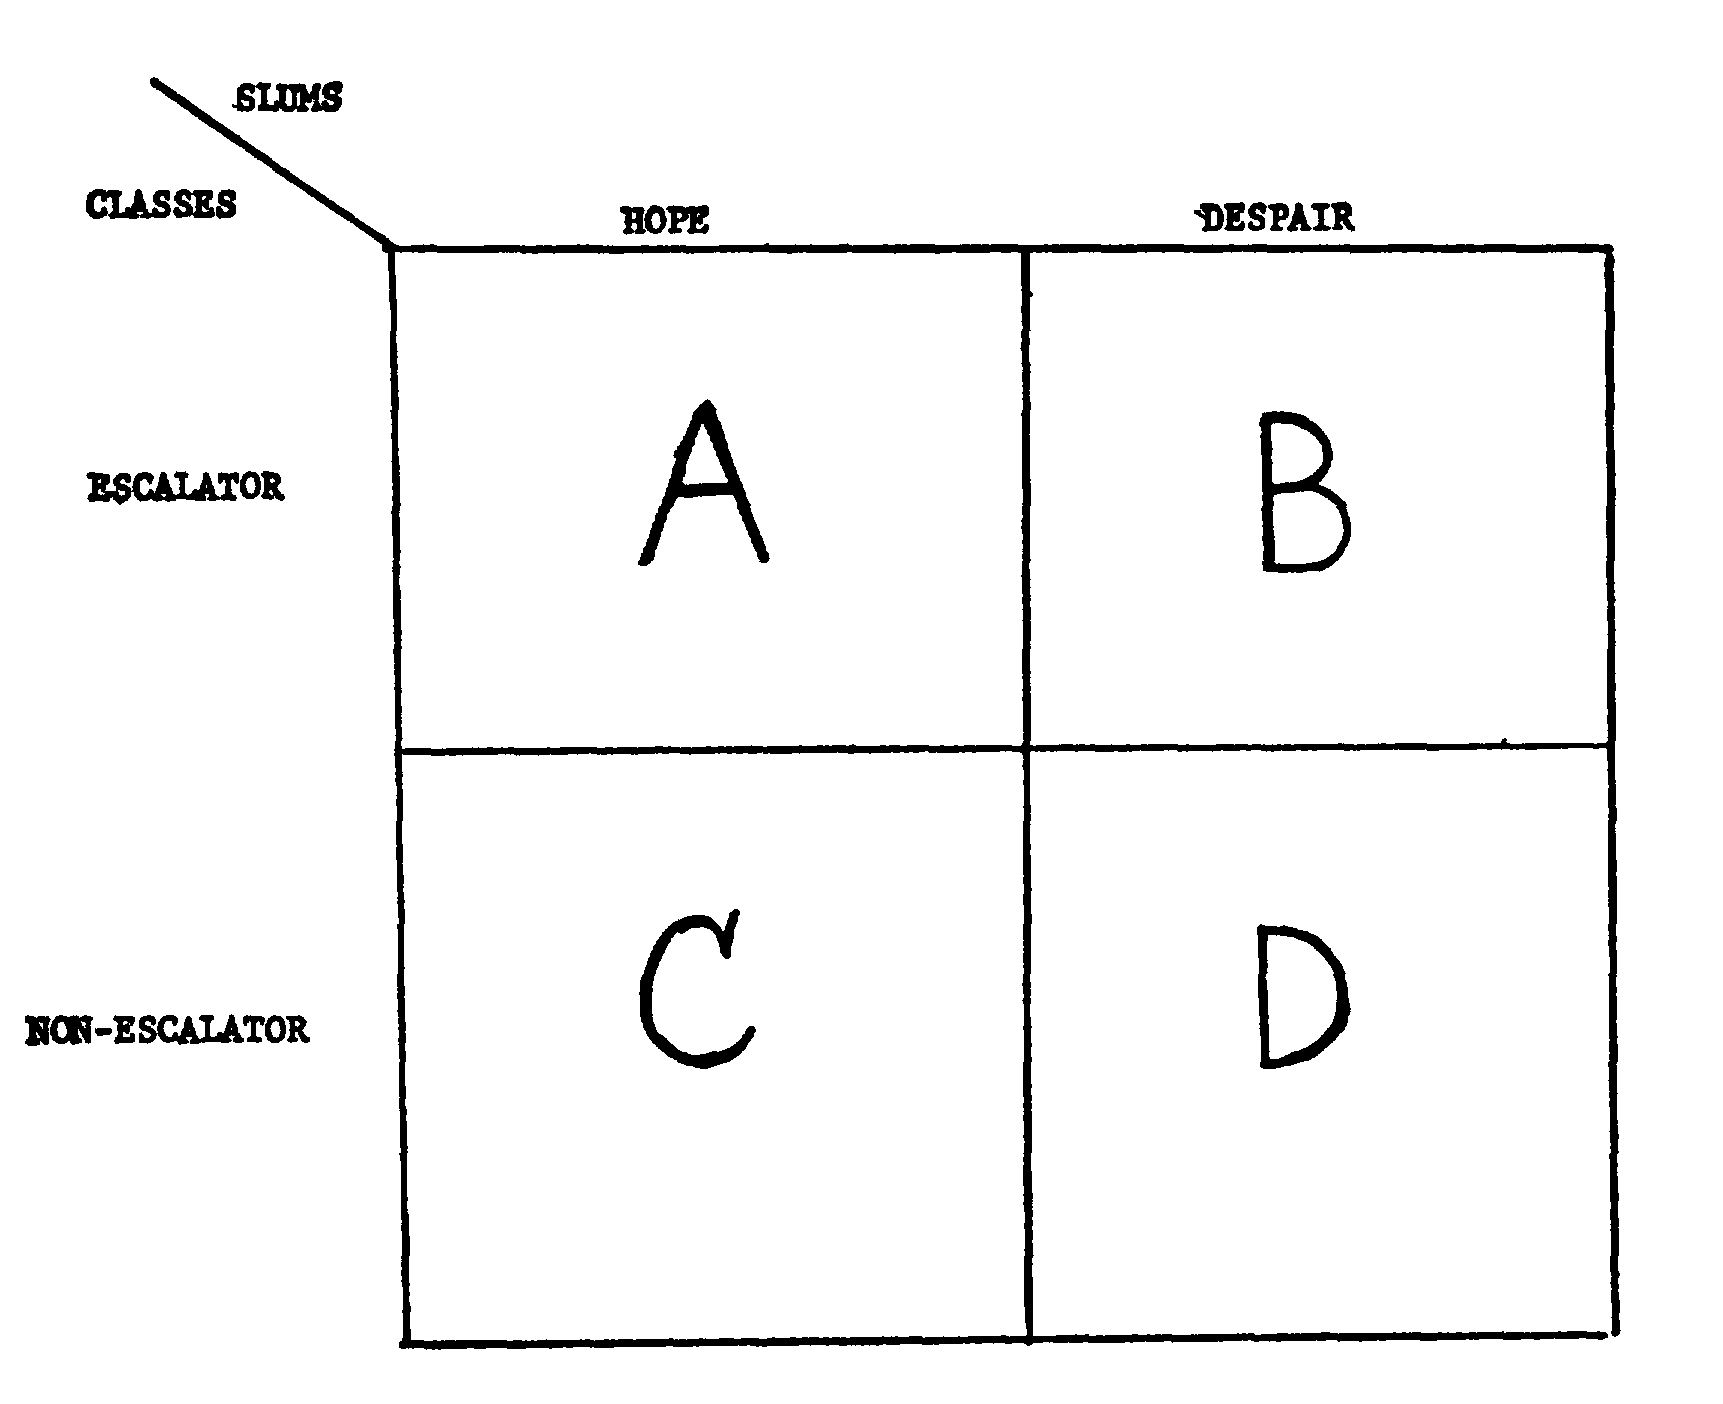
\includegraphics[width=0.4\textwidth]{images/img}
    \caption{Slums classification. Reprinted from “A theory of slums,” by  C. J. Stokes, 1962, Land economics, vol. 38, p. 189. Copyright Year by JSTOR.}
    \label{fig:slums_classification}
\end{figure}

The hope factor is related to the reason of the settlement, whether it is done by necessity or in search of better opportunities. While the escalator factor is related to the integration of slum dwellers for reasons of culture, religion or race.\\

In practical terms, most type A slums are the result of migrations of people from the same country who have some economic capacity. While the slums belonging to the other types is formed by people of very different origins or with no economic capacity. This causes that differences can be appreciated in the ordering of the constructions according to the type of slum. For instance, in the slums of type A we could find a kind of linear arrangement of the constructions because people living there have the intention to stay there for a while, but in slums of type D the constructions seem to be more random because their dwellers were probably settle for need, see figure \ref{fig:slumD} and figure \ref{fig:slumA}.\\ \

\begin{figure}[h]
    \centering
    \begin{minipage}{0.40\linewidth}
        \centering
        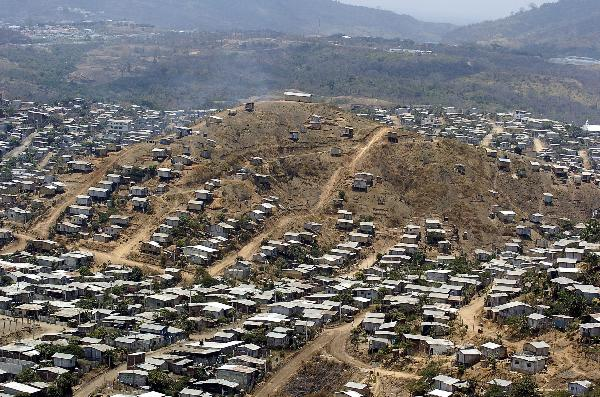
\includegraphics[width=0.95\textwidth]{images/slum_a.jpg}
        \caption{Slum of type D. By Institute for Housing and Urban Development Studies, CC BY-SA 3.0, https://commons.wikimedia.org/w/index.php?curid=34389333}
        \label{fig:slumD}
    \end{minipage}%
    \begin{minipage}{0.40\linewidth}
        \centering
        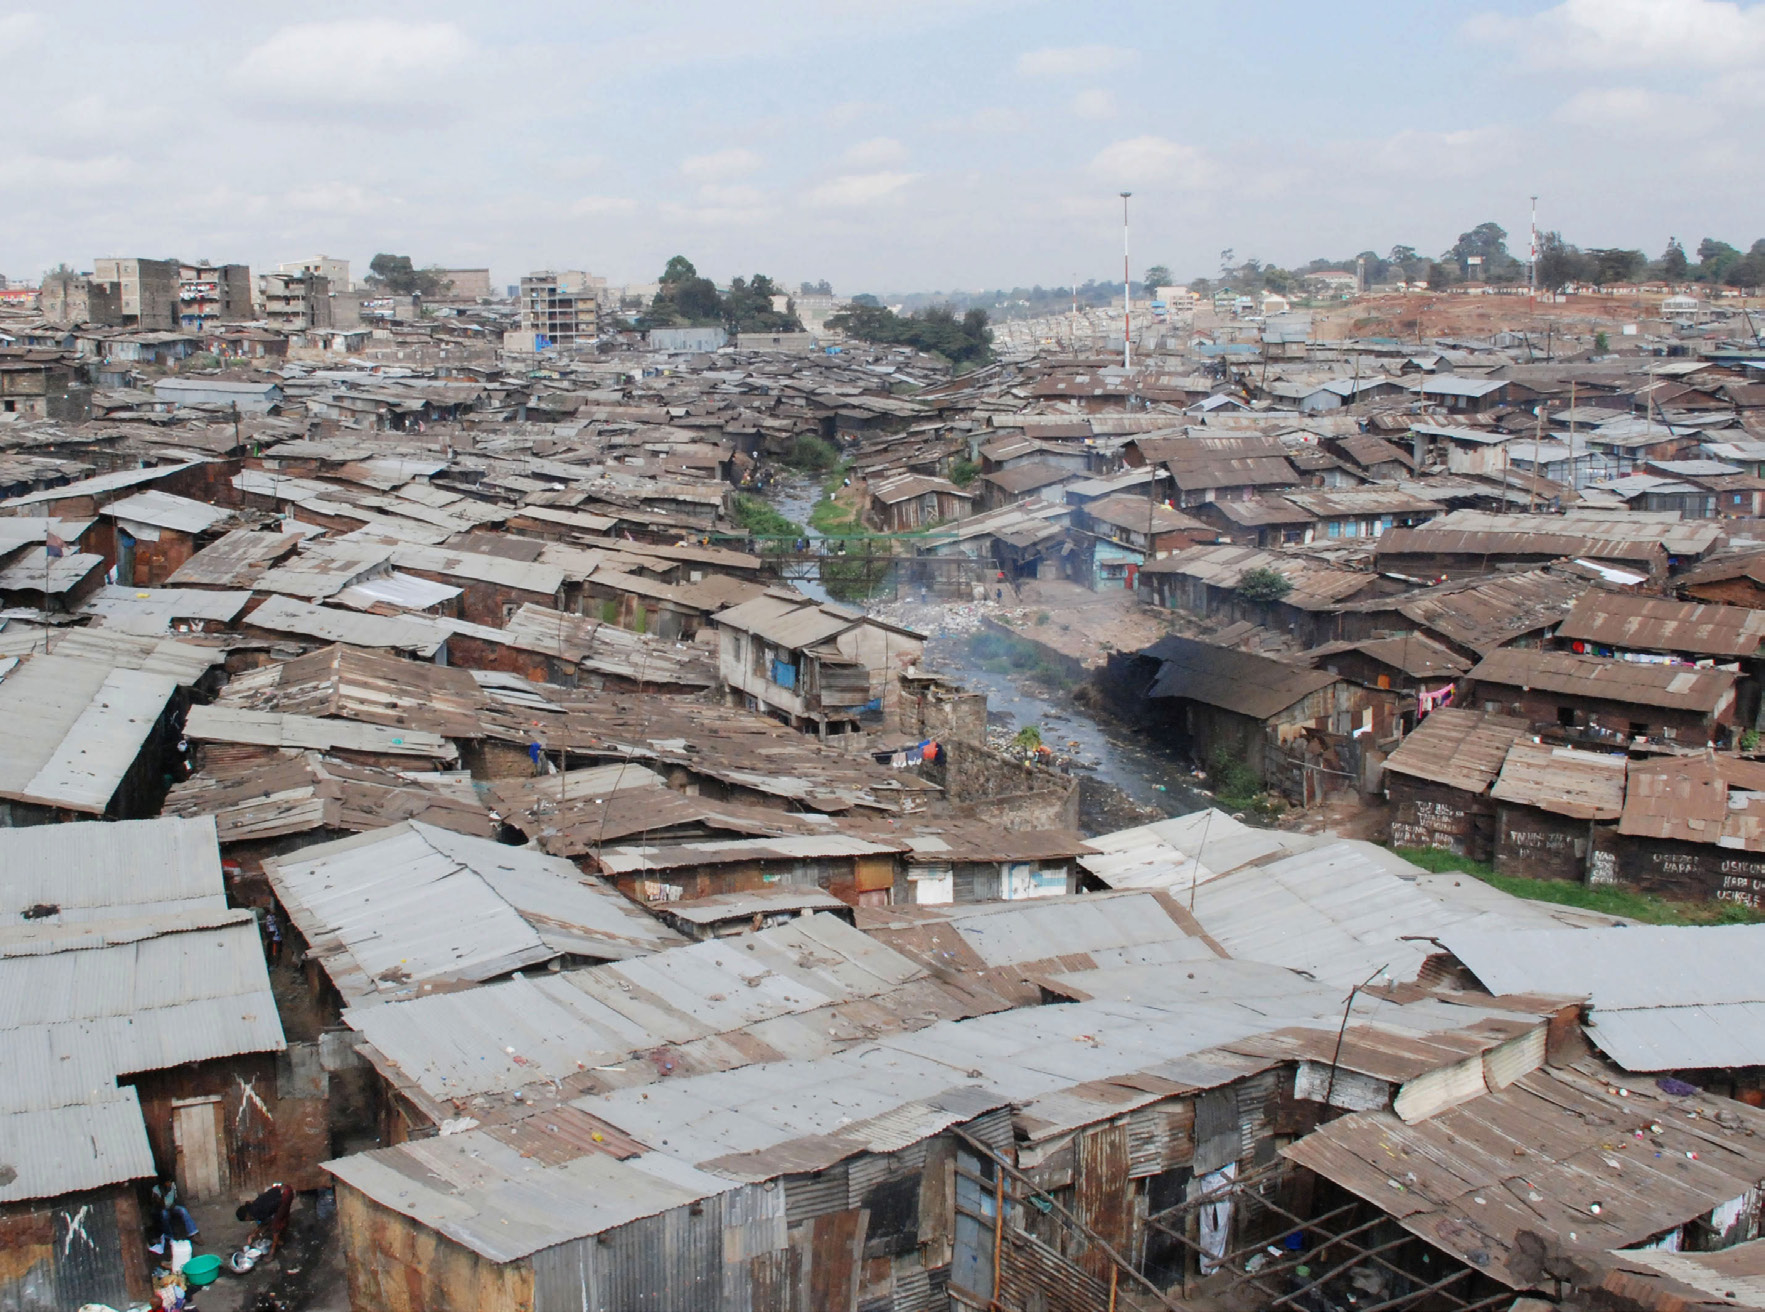
\includegraphics[width=0.8\textwidth]{images/slum1.png}
        \caption{Slum of type A. Reprinted from “SLUM ALMANAC 2015/2016: Tracking Improvement in the Lives of Slum Dwellers,” by  UN-Habitat, 2016, Participatory Slum Upgrading Programme, p. 9. Copyright Year by UN-Habitat/Julius Mwelu.}
        \label{fig:slumA}
    \end{minipage}
\end{figure}


Remark that since the proposed factors for the classification are qualitative, a slum could be of type A but still have certain similarities with those of other types.

\subsubsection{Slums in Guayaquil}

According to Camila Mackliff, 59 \% of Guayaquil's surface is occupied informally \cite{cam_mac}. This is due to the fact that the growth of the city took place through the informal accumulation of people who migrated to the city, at first, fleeing the adverse conditions generated by the economic crises that occurred in the history of Ecuador but now to take advantage of the economic conditions provided by the city with the largest maritime port in Ecuador ().\\

Given the current conditions of creation of the slums it can be said that most of the new slums in Guayaquil are of type A. In particular, the \emph{Ciudad de Dios} neighborhood, which in 2010 was an area with a lot of vegetation but now can be found spontaneous constructions, see figure(). An important characteristic of the informal settlements of Guayaquil is that normally the lands where they are located belong to land traffickers, which means that the location of the houses is carried out in lots and that it is not completely random().

\begin{figure}[h]
    \centering
    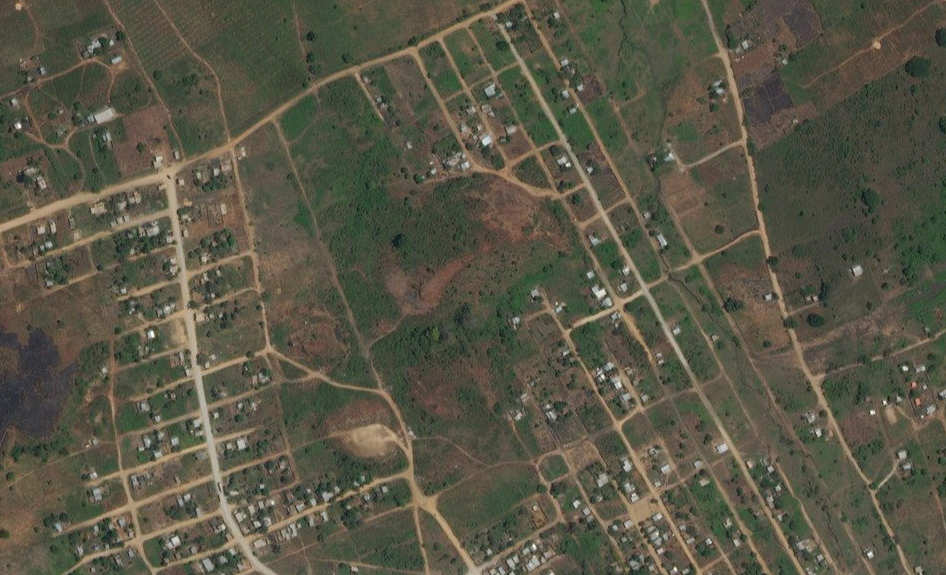
\includegraphics[scale = 0.31]{images/slum2010}
    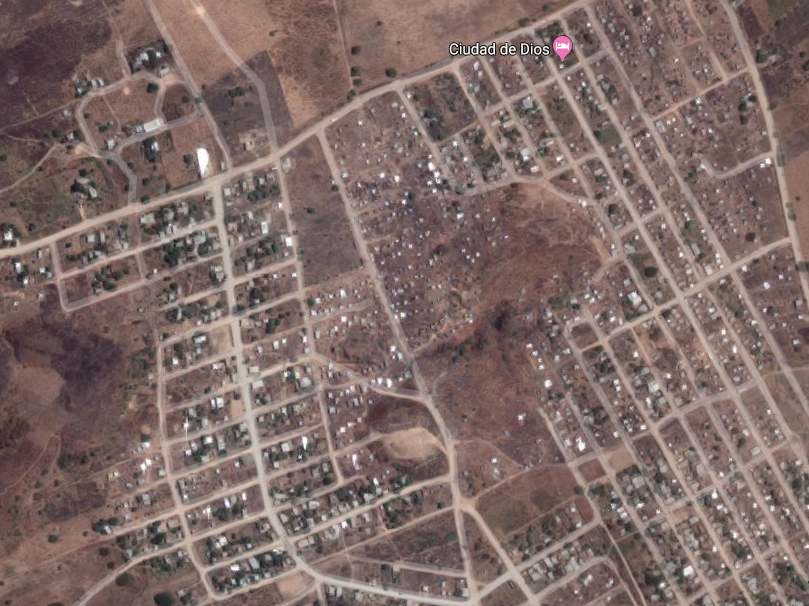
\includegraphics[scale = 0.22]{images/slum2019}
    \caption{Caption}
    \label{fig:my_label}
\end{figure}

Bertaud is a detractor of the use of strategies guided by topological algorithms to restructure the slums. Because usually the solutions that involve the construction of roads need space, which will be obtained through the eviction of some inhabitants\cite{Ornes9686}. However, the reality of slums in Ecuador is that they are not as dense as those that can be found in other countries such as India for example. This makes it easier to find ways to create these roads. 

\subsubsection{Upgrade Slums}


\subsection{Topological Graph Theory}
Before showing the results of the study of the Topology of the Cities, it is necessary to review some general concepts of the theory of topological graphs. Our principal resources are \cite{gross2009topics}, \cite{bonnington2012foundations}, \cite{gross1987topological} and \cite{richeson2008euler}.\\

\begin{definition}[Graph]
A graph $G$ is a pair of sets $(V , E)$, where $V$ is a finite non-empty set of elements called vertices, and $E$ is a finite set of elements called edges, each of which has two associated vertices (which may be the same).
\end{definition}

The sets $V$ and $E$ are the vertex-set and edge-set of $G$, and are sometimes denoted by $V(G)$ and $E(G)$. The order of $G$ is the number of vertices, usually denoted by n, and the number of edges is denoted by m.

\begin{definition}[Walk]
A walk in a graph is a sequence of vertices and edges $v_0, e_1, v_1, \dots, e_k, v_k$, in which each edge $e_i$ joins the vertices $v_{i-1}$ and $v_i$. This walk goes from $v_0$ to $v_k$ or connects $v_0$ and $v_k$, and is called a $v_0-v_k$ walk.
\end{definition}

\begin{itemize}
    \item a path is a walk in which no vertex is repeated;
    \item a cycle is a non-trivial closed walk in which no vertex is repeated, except the first and last;
    \item a trail is a walk in which no edge is repeated;
    \item a circuit is a non-trivial closed trail.
\end{itemize}

\begin{definition}[Surface]
A (topological) surface is a topological space in which every point has an open neighbourhood homeomorphic to some open subset of the Euclidean plane $E_2$.
\end{definition}

A sphere and a torus are examples of closed surfaces. They have no punctures, they do not run off to infinity, and they do not have any sharp boundaries. Sometimes we want to consider surfaces that are not closed. A disk and a cylinder are examples of surfaces with boundary. A surface with boundary is still locally 2-dimensional, except that it may have one or more 1-dimensional boundary curves.\\

There are two kinds of closed surfaces, orientable and nonorientable. A surface is $orientable$ if a positive sense of rotation (say, clockwise) can be made around all points consistently, and is $non-orientable$ otherwise. The sphere, the torus, the double torus, the triple torus, and so on, are orientable. They are commonly denoted $S_0$, $S_1$, $S_2$, $S_3$, ... Moreover, every closed connected orientable surface is homeomorphic to one of them. Another characterization of the closed orientable surfaces is that each one can be obtained by adding some handles to a sphere. Adding one handle yields S1, adding two yields S2, and so on.\\

To formalize the notion of a drawing without crossings, we define an "imbed-ding"\\
  
\begin{definition}[Embedding of a Graph on a Surface]
An embedding of a graph $G$ on a surface $S$ is an one-to-one mapping of the vertices of G into that surface and a mapping of the edges of G to disjoint simple open arcs, so that the image of each edge joins the images of its two vertices and none of the images of the edges contains the image of a vertex.
\end{definition}

The plane is not closed, of course but since it differs from the sphere by only a single point, it follows that a given graph can be imbedded in the plane if and only if it can be imbedded in the sphere.\\

A $region$ of an embedded graph $G$ is a maximal connected set of points in the relative complement of $G$ in the surface; note that one region is unbounded. The topological closure of a region (that is, the region together with the vertices and edges of $G$ on its boundary) is a $face$.

\begin{definition}[Cellular Embedding]
 An embedding is $cellular$ if every region is homeomorphic to an open disc.
\end{definition}

\begin{theorem}[Euler’s formula]
    If a simple graph $G$ has a cellular embedding in a surface $S$ with $n$ vertices, $m$ edges and $r$ regions, then
    $n-m+r=2-2h,$ where h is the genus of the surface $S_h$.
\end{theorem}

The number associated with $S$ in this theorem is called its Euler characteristic.

\begin{definition} [Genus of a Graph]
The $genus$ $\gamma(G)$ of a graph $G$ is the minimum genus of a surface in which the graph can be embedded – that is, the minimum number of handles that need to be added to the sphere for $G$ to be embeddable.
\end{definition}

A connected graph of genus 0 is said to be planar. In general, a graph is planar if all of its components are planar. Thus, non-empty connected planar graphs are the graphs imbeddable in the sphere. They are the ones that underlie spherical gems. In general, the determination of the genus of a graph is  an unsolved problem. 

\begin{definition}[Poincar\'e Dual Embedding]
The \emph{Poincar\'e dual embedding} for a cellular graph embedding $G\xrightarrow{}S$(called \emph{the primal embedding} in this context) is constructed as follows:
    \begin{itemize}
        \item in the interior of each primal region, a \emph{dual vertex} is drawn;
        \item through each primal edge, a \emph{dual edge} is drawn joining the dual vertex on one side of the edge to the dual vertex on the other (thus, a loop whenever the same primal region lies on both sides of that primal edge);
        \item if the surface $S$ is oriented, then in the dual embedding, the orientation is reversed.
    \end{itemize}
\end{definition}

A famous graph is the Birkhoff diamond, it is used to study the colorability of some graphs\cite{tilley2018birkhoff}. This graph is show in fig.().

\begin{figure}[H]
    \centering
		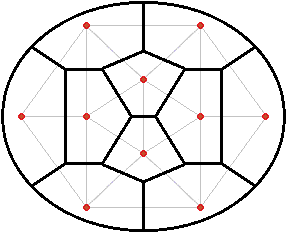
\includegraphics[scale=0.75]{images/Birkhoff_diamond.png}
    \caption{Caption}
    \label{fig:my_label}
\end{figure}

\subsection{Topology of the City}
The topology of cities/neighborhoods can be understood as the topological relationship between the two main components of the city: its streets and its buildings. This is the reason why it is necessary to understand the topology of the access systems and the topology of the constructions, to then see how they are related according to each city.

\subsubsection{Topology of Access System}
The set of paths and roads of any city is called urban access system. The access system has the property of be \textbf{path-connected}, i.e., any two points in this surface can be connected traveling on the surface. Moreover, access systems are \textbf{orientable}, \textbf{2-dimensional surface} and \textbf{compact}. This properties are related with the following facts: there is a global definition of up from down, we can only move on road and path surfaces and the surface is finite.\\

Moreover, the urban access system is a 2D surface with both \textbf{internal} and \textbf{external boundaries}: The limit of the city is the external boundary, while boundaries between accesses and each places are the internal boundaries. So, for a city with $b$ blocks there are $b$ internal boundaries and one external boundary so that the total number of boundary components, $B$, is $B = b+1$. In this sense, a city subsection is define as a set of contiguous city blocks and surrounding access system, including an external boundary that defines the physical limits of the subsection, see fig.(). When a subsection includes all blocks it is equivalent to the city, and shares its entire access system.\\

%figureofaccess system

The authors in \cite{bre} show that the topology of  the access system of a city with $b$ blocks is equivalent to the topology of a sphere with $b+1$ disks removed. In consequence, urban access systems are topologically equivalent if and only if they have the same number of blocks. Moreover, if we use a graph representation of the urban access system ($Y$), as the suggested in \cite{por}, where edges correspond to roads or paths, and nodes correspond to their intersections, $Y$ has the same Euler characteristic as the urban access system, $\chi(Y) = 1 - b$.\\

This deductions are summarize in the following theorem and corollaries:\\
\begin{theorem}[Topological Classes of Urban Access System]
The access system of any city with $b$ blocks is topologically equivalent to a sphere with $B=b+1$ disks removed.
\end{theorem}
\begin{proof}
The proof of this theorem is based on the fact that the surfaces with boundaries can be constructed by removing open discs from the surfaces without boundary. Therefore, as the access system is orientable, 2-dimension and has genus zero; it is topologycal equivalent to a sphere but with b+1 open discs removed. 
\end{proof}

The proof of the following four corollaries are trivial by the definition of topological equivalence and the previous theorem. So we proceed with the demonstration of the fifth corollary.

\begin{corollary}
    For any value of $b$, two cities with $b$ blocks have access systems that are topologically equivalent, since both cities’ access systems are topologically equivalent to a sphere with $b+1$ disks removed.
\end{corollary}

\begin{corollary}
    Any subsection of one city with $b$ blocks has an access system that is topologically equivalent to that of another subsection of another city with $b’$ blocks,if and only if $b=b’$.
\end{corollary}

\begin{corollary}
    The access system of an entire city with $b$ blocks is topologically equivalent to a subsection of any other city with the same number of blocks.
\end{corollary}

\begin{corollary}
    Urban Access Systems are topologically equivalent if and only if they have the same number of blocks. 
\end{corollary}

\begin{corollary}
    A 1-complex graph representation of an urban access system with $b$ blocks, where edges correspond to road and path centerlines and nodes correspond to their intersections, called the urban access network, $Y$, has the same Euler characteristic as the urban access system, $\chi(Y)=1-b$. 
\end{corollary}
\begin{proof}
	Let's compute the Euler characteristic of a general surface $S$ with $B$ boundaries.\\
	
	First define a surface $C$, where $S^*$ corresponds to $S$ with all the $B$ boundaries patched by disks.\\
	
	Then,	$\chi(S^*)=\chi(S)+B*\chi(Disk)$.\\
	Since, $\chi(Disk)=1$ and $\chi(S^*)=2$ because $S^*$ is a sphere.\\
	
	$\chi(S)=2-(1+b)=1-b$.\\
	
	On the other hand, a 2-complex planar graph has $\chi=v-e+f=2$, while a 1-complex planar graph has $\chi=v-e$. Let be $Y_2$ a 2-complex graph representation of the urban access system, then, $Y_2$ has one face per each boundary so $f=b+1$.\\
	
	Then,	$\chi(Y_2)=v-e+f=2$\\
	$v-e=2-f=1-b=\chi(Y)$\\
	Therefore, $\chi(Y)=\chi(S)=1-b$
\end{proof}


\subsubsection{Topology of City Blocks}

Brelsford et. al. use the general term parcel in \cite{bre} to denote the decomposition of the city block land area into separate units: these are buildings, or more generally, separate land holdings and include public places that are not accesses. When a parcel is adjacent to the access network is said that this parcel is accessible. In the case where the parcel is not adjacent to the access network is internal to the block, this implies that its access is mediated through other parcels. However, interior parcels can be connected to the urban access system by converting edges in the $S_0$ graph from parcel boundaries to roads, where the edges of $S_0$ correspond to the boundaries of each parcels and its nodes to their intersections, see fig().\\

One characteristic of mostly planned neighborhood is that all their parcels are accessible, since slums are more likely to have inaccessible parcels \cite{unh}. Then, the connectivity of the neighborhoods seems to be useful to look at them. This characteristic of the neighborhood can be analyzed using a metric $k_{max}$, called block complexity, which measure the connectivity of a city block. Additionally, they have show that it is possible to find $k_{max}$ by iterating the construction of weak dual graphs to $S_0$; the weak dual graph of $S_0$ is $S_1$, where each parcel becomes a node and adjacency becomes and edge. This procedure should be done iteratively ($S_{k-1}\longrightarrow S_k$) until there is not more parcels in the graph $S_k$. Moreover, they found that the complexity of universally accessible block (blocks with all parcels accessible) is $k \leq 2$, while non-universally accessible blocks (blocks with interior parcels) will have $k>2$. Furthermore, a block S is universally accessible if and only if $S_2$ is a tree. And, if a parcel is represented with a node in the $S_k$ graph, at least $\frac{k-1}{2}$ parcel boundaries must be crossed in order to reach it from the nearest section of the access system.\\

Finally, in the minimal set of additional roads necessary to have a universal accessible block there will be no loops. Thus, newly constructed roads in the minimal set of accesses form a tree or set of trees (culs-de-sac). This feature is interesting because loopless configurations are seem in river basins where every spanning tree is exactly a local minimum of total energy dissipation \cite{and}.\\

These statements are shown in more detail below.

\begin{definition}
A block $S$ is called universally accessible if every parcel within $S$ borders a road.  Otherwise, $S$ is not universally accessible.
\end{definition}

\begin{definition}[minimal set of accesses]
Interior parcels can be connected to the urban access system by converting edges in the $S_0$ graph from parcel boundaries to roads.  The minimal set of additional roads necessary to connect a given parcel to the road system is the set of edges with the shortest total length such that at least one node contained in the set of edges to be converted is part of an existing road, and at least one node is part of the face in $S_0$ that surrounds the parcel.
\end{definition}

\begin{definition}
In a graph $G$, a cycle is a collection of $m$ vertices and $m$ edges arranged so that each vertex has exactly two edges incident to it, where $m \ge 3$.
\end{definition}

\begin{definition}
A face of a planar graph is a maximal region in the plane that contains no edge or vertex of the graph.
\end{definition}

\begin{definition}[Weak Dual Graphs]
For each bounded face of $S_0$, we assign a vertex in $S_1$. Two vertices of $S_1$ have an edge between them if and only if the faces of $S_0$ they represent share a common border of at least one edge in $S_0$. Then, $S_1$ is the weak dual graph of $S_0$. For a block $S$, we may then assign a stage $k$ graph, $S_k$, defined recursively by repeating the process used to construct $S_1$ from $S_0$ on the stage $k-1$ graph $S_{k-1}$.
\end{definition}

\begin{figure}[H]
    \centering
    \begin{minipage}{.33\textwidth}
        \centering
        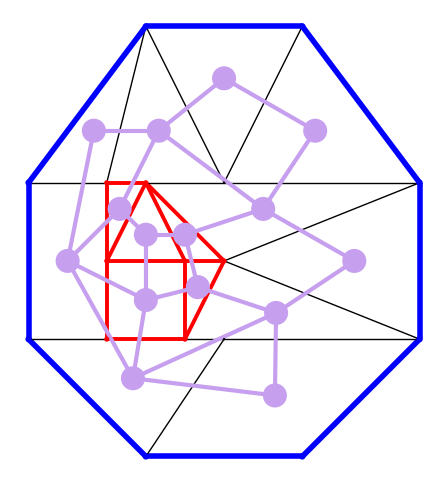
\includegraphics[width=0.75\textwidth]{images/dual1}
        \caption{$dt=0.1$}
        \label{fig:prob1_6_2}
    \end{minipage}%
    \begin{minipage}{.33\textwidth}
        \centering
        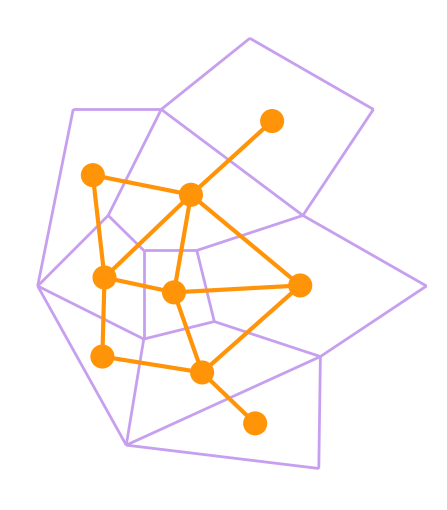
\includegraphics[width=0.75\textwidth]{images/dual2}
        \caption{$dt=0.1$}
        \label{fig:prob1_6_2}
    \end{minipage}%
    \begin{minipage}{.33\textwidth}
        \centering
        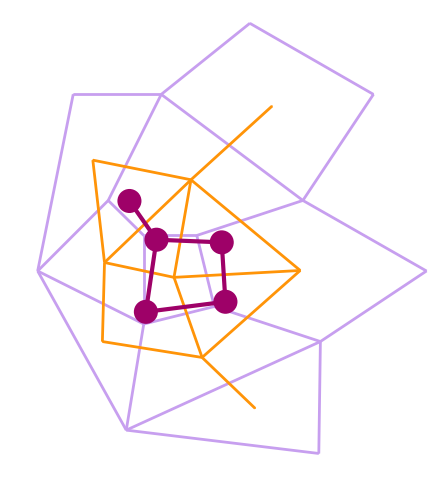
\includegraphics[width=0.75\textwidth]{images/dual3}
        \caption{$dt=0.1$}
        \label{fig:prob1_6_2}
    \end{minipage}
\end{figure}


\begin{definition}
A vertex $v$ of a graph $G$ is called an $interior\ vertex$ if there exists a cycle surrounding $v$ so that deleting this cycle from $G$ results in either:
    \begin{enumerate}
        \item Two connected components, one of which contains vertex $v$ and all of its incident edges,or
        \item Just the vertex $v$ and its incident edges.
    \end{enumerate}
\end{definition}

\begin{definition}
A graph $G$ is called a $tree$ if $G$ contains no cycles. 
\end{definition}

\begin{definition}[block complexity]
The $complexity$ of the block $S$ is the smallest positive integer $k$ such that $S_k$ is a tree. Every block will be characterized by a positive, discrete value of this complexity. \\
The complexity of universally accessible blocks is $k \leq 2$. Non-universally accessible blocks will have $k>2$.
\end{definition}

\begin{theorem}
    A block $S$ is universally accessible if and only if its stage-two graph, $S_2$, is a tree.
\end{theorem}
\begin{proof}
Let's assume that $S_2$ is not a tree.  This means that there exists an interior face of $S_2$ whose boundary is a cycle $\sigma$ consisting of $m$ vertices${x_1, x_2, ...,x_m}$ of $S_2$ and $m$ edges. Each vertex $x_i$ in $\sigma$ represents a face $f_i$ of $S_1$, where face $f_i$ shares a common edge with face $f_{i-1}$(mod m)and face $f_{i+1}$(mod m). Furthermore, each of these shared edges is incident to a vertex $v$ of $S_1$ that represents the interior face of $S_2$. Thus, the cycle $\sigma$ in $S_2$ corresponds to a subgraph of $S_1$ consisting of the $m$ faces, ${f_1, f_2, ..., f_m}$ arranged in a circle around the vertex $v$. This means that vertex $v$ is an interior vertex of $S_1$, so it corresponds to a parcel of the block $S$ that does not border a road. This shows that block $S$ is not universally accessible. Now, we will prove that if a block $S$ is not universally accessible, its stage two graph, $S_2$, is not a tree. We assume that there exists a parcel $n$ of a block $S$ that does not border a road.  Thus, there is a vertex $v_n$ of $S_1$ corresponding to parcel $n$ that is an interior vertex of $S_1$. Consider the subgraph $V_1$ of $S_1$ consisting of a minimal cycle surrounding vertex $v_n$, vertex $v_n$ itself and all edges incident to vertex $v_n$. Now, we consider the subgraph $V_2$ of $S_2$ that represents $V_1$. $V_2$ will contain one vertex for each face of $V_1$ connected by one edge representing each edge incident to vertex $v_n$.We conclude that the subgraph $V_2$ of $S_2$ is a cycle with $m$ vertices, where $m$ is the degree of vertex $v_n$ in $S_1$.This says that the stage two graph of $S$ contains a cycle, and is therefore not a tree.
\end{proof}

\begin{theorem}
    If a parcel is represented with a node in the $S_k$ graph, at least $\frac{k-1}{2}$ parcel boundaries must be crossed in order to reach it from the nearest section of the access system.
\end{theorem}
\begin{proof}
For any parcel $n$ of block $S$, the minimum number of parcel boundaries that must be crossed in order to reach a road is represented by the minimum number of edges necessary to form a path from $v_n$, the vertex representing $n$ in the $S_1$ graph, to an exterior vertex of $S_1$.\\

Observe that, in the algorithm for creating the $S_k$ graph of a block $S$, parcels of $S$ are represented by faces of $S_k$ when $k$ is even and nodes of $S_k$ when $k$ is odd. Furthermore, for even $k$, if a face of $S_k$ touches an exterior vertex, that face is represented by an exterior vertex in $S_{k+1}$. Finally, observe that, for odd $k$, parcels represented by an exterior vertex of $S_k$ are not represented at all in $S_{k+1}$.\\

Therefore, suppose a parcel $n$ requires a path of length $l$ to connect vertex $v_n$ to an exterior vertex in $S_1$. It is clear that in $S_3$, the path from $v_n$ to an exterior vertex will have length $l-1$,and so on. The vertex $v_n$ will thus be an exterior vertex of the graph $S_{1+2l}$. Therefore, we see that, if vertex $v_n$ appears in graph $S_k$, then $k\leq 1+2l$, which says that $\frac{k-1}{2}\leq l$.
\end{proof}

\begin{theorem}
    There will be no loops in the minimal set of additional roads necessary to connect all interior parcels to a road. Thus, newly constructed roads in the minimal set of accesses form a tree or set of trees (culs-de-sac).
\end{theorem}
\begin{proof}
We may consider the access network of a given block as a subgraph of the stage zero graph $S0$. In order to connect all parcels to a road, we consider parcel boundaries, which are represented by interior edges in $S0$. We may then choose a set of such edges of $S0$ to represent additional segments of road needed to ensure that the block is universally accessible. There will be several choices for this set of additional roads; we choose the one that has the fewest total geometric length of edges (minimalset of accesses).\\

Suppose that there exists a block for which the minimal set of additional roads is not a tree or set of trees. Let $M$ denote the subgraph of $S0$ consisting of edges belonging to the minimal set of roads along with the nodes incident to these edges. We are assuming that there is at least one cycle in $M$. Every face of $S0$ representing an interior parcel must share at least one node with $M$ in order for every parcel to be accessible via existing or new paths. However, all connected planar graphs have a spanning tree, which is a subgraph containing all nodes of the graph but no cycles. Then, we let $M’$ be the subgraph of $M$ consisting of spanning trees for each component of $M$. Thus, every face of $S0$ representing an interior parcel will share a node with $M’$, making every parcel accessible via existing or new roads, but $M’$ has strictly fewer edges than $M$, as it is a subgraph containing no cycles. This contradicts the choice of $M$ as minimal. Therefore, the set of newly constructed roads must form a tree or set of trees
\end{proof}

\subsection{Topological optimization: Minimal Neighborhood Reblocking}

 In \cite{bre}, the authors define this topological optimization problem in two different ways. The first, a strict optimization that is too rigid for practical use. The second, a statistical optimization that is more flexible and can be the basis for practical neighborhood upgrading tools.\\

The strict optimization approach seeks to find the smallest possible configuration of the streets to ensure that each interior parcel is connected to the access system. Although this strategy found the best solution, the computational complexity grows in a combinatorial way according to the number of parcels that are considered. This is because there may be solutions with shorter length if they are considered a pair, trio, etc. of internal plots together. In consequence this approach is not practical for real situations.\\

The statistical optimization starts from the fact that some paths, despite not being the most optimal, have characteristics that may be interesting for us. Then this technique allows to use additional data to the problem of strict optimization, such as the price of building new streets or how straight the roads are. As the criterion of the cost of construction of streets is a function of the street length, it is understandable why this strategy of optimization delivers as a result that the smaller roads must be built more likely.\\

The approach developed by Brelsford et. al. to deal with blocks within large number of parcels consists in the following steps. First, find the solution of strict optimization for an interior parcel. Then, define a set of feasible solutions adding $n$ alternative paths to connect the parcel with the access system. This process must be repeated for the rest of interior parcels. Then, use the defined probability function for statistical optimization to select a single path from our set of feasible path solutions. After adding the selected path to the access system, the information of the interior parcels is updated and the whole process is repeated until there are no more interior parcels, i. e., the graph $ S_2 $ is a tree.

\section{Implementation of the Approach}
The approach was implemented and tested using two examples: an academic one and a real life one. The real life implementation was developed using a zone of the neighborhood \emph{Ciudad de Dios} in Guayaquil.\\

The objective to use an academic example is to recreate the proposal described in [], and in this way to be able to verify the different solutions that the algorithm gives us depending on the type of optimization used, i.e., strict optimization(piecewise) or statistical optimization. Moreover, we should be able to verify the construction of the dual graph for a block with interior parcels as the theory related with it.\\

On the other hand, the motivation to use a real life example is to show that this proposal is viable to be used in the context of the Ecuadorian slums.

\subsection{Implementation on Academic Example}
The academic example consists in 15 parcels, where 10 of them are exterior parcels and five are interior parcels, see figure().\\

\begin{figure}[H]
    \centering
    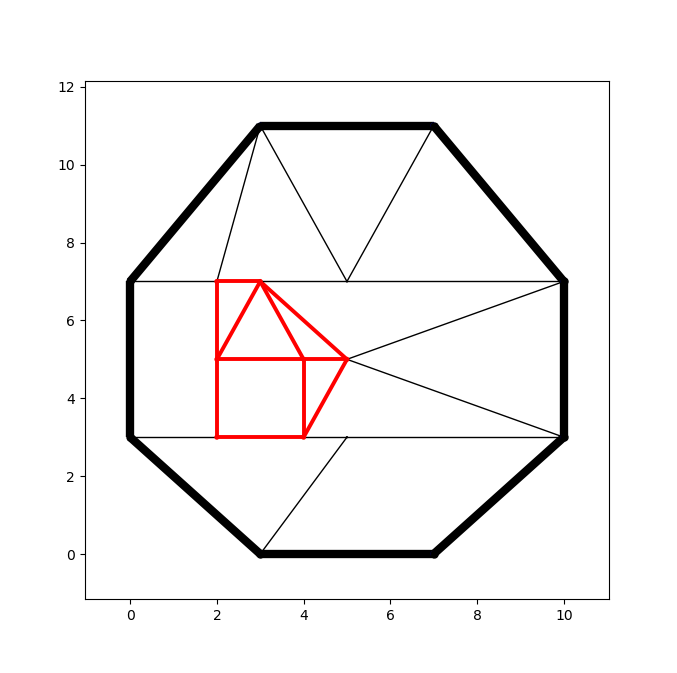
\includegraphics[width=0.50\textwidth]{images/Figure_1.png}
    \caption{Caption}
    \label{fig:my_label}
\end{figure}

From this example is possible to realize that the corresponding $S_2$ (see figure ())graph has a loop, which means that our block is not universally accessible. Therefore, we can use the approach in order to upgrade his interior parcels to external parcels.\\


\begin{figure}[H]
    \centering
    \begin{minipage}{.33\linewidth}
        \centering
        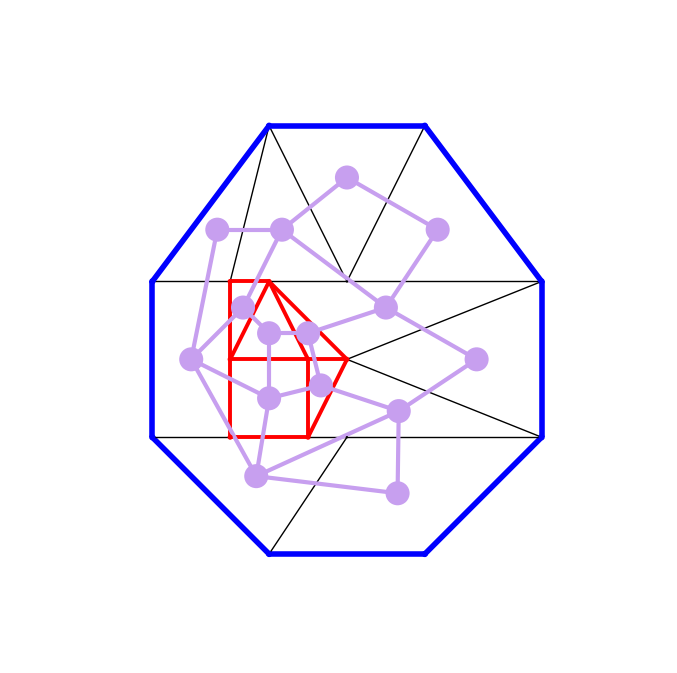
\includegraphics[width=1\textwidth]{images/Figure_2.png}
        \caption{$dt=0.1$}
        \label{fig:prob1_6_2}
    \end{minipage}%
    \begin{minipage}{.33\linewidth}
        \centering
        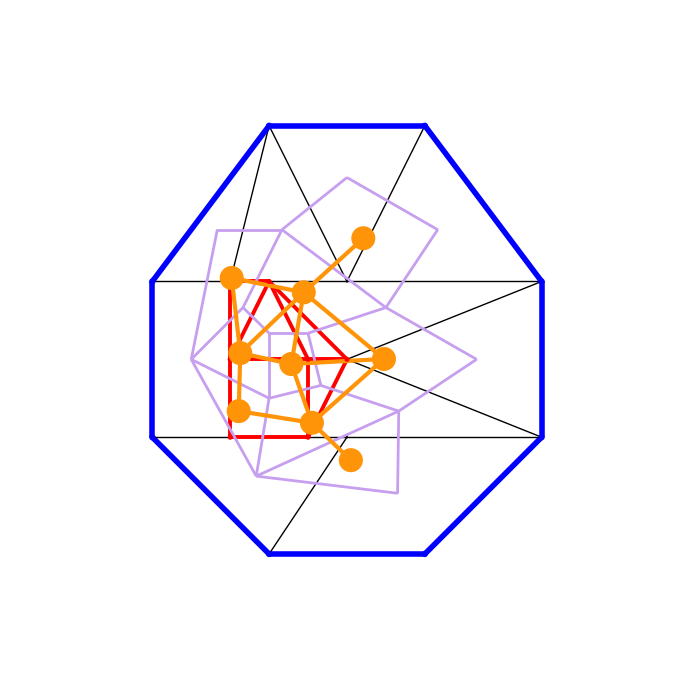
\includegraphics[width=1\textwidth]{images/Figure_4.png}
        \caption{$dt=0.1$}
        \label{fig:prob1_6_2}
    \end{minipage}%
    \begin{minipage}{.33\linewidth}
        \centering
        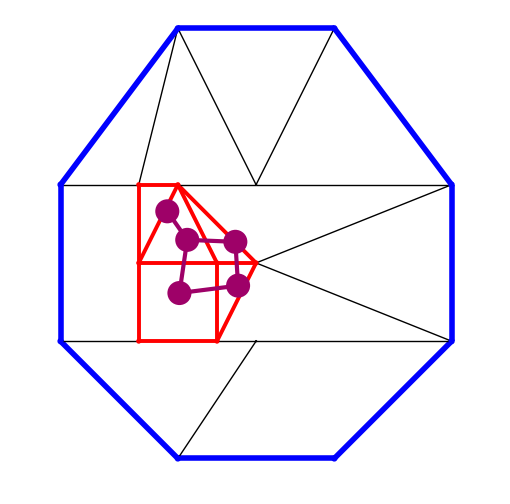
\includegraphics[width=1\textwidth]{images/dual4.png}
        \caption{$dt=0.1$}
        \label{fig:prob1_6_2}
    \end{minipage}
\end{figure}
 
Using the strict optimal (piecewise) algorithm in our academic example, the solution is constructed adding the smallest road in order to change an interior parcel into a exterior parcel in each iteration, see figure ().

\begin{figure}[H]
    \centering
    \begin{minipage}{.4\linewidth}
        \centering
        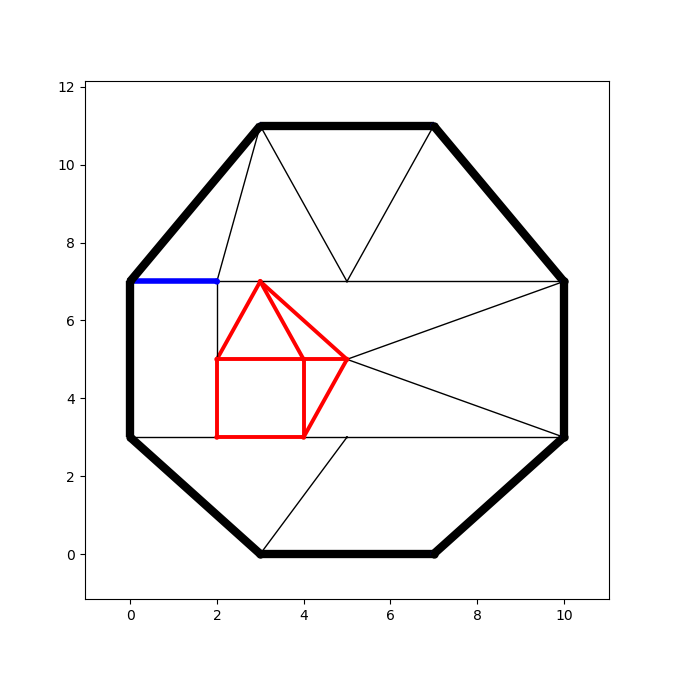
\includegraphics[width=1\textwidth]{images/Figure_5.png}
        \caption{$dt=0.1$}
        \label{fig:prob1_6_2}
    \end{minipage}%
    \begin{minipage}{.4\linewidth}
        \centering
        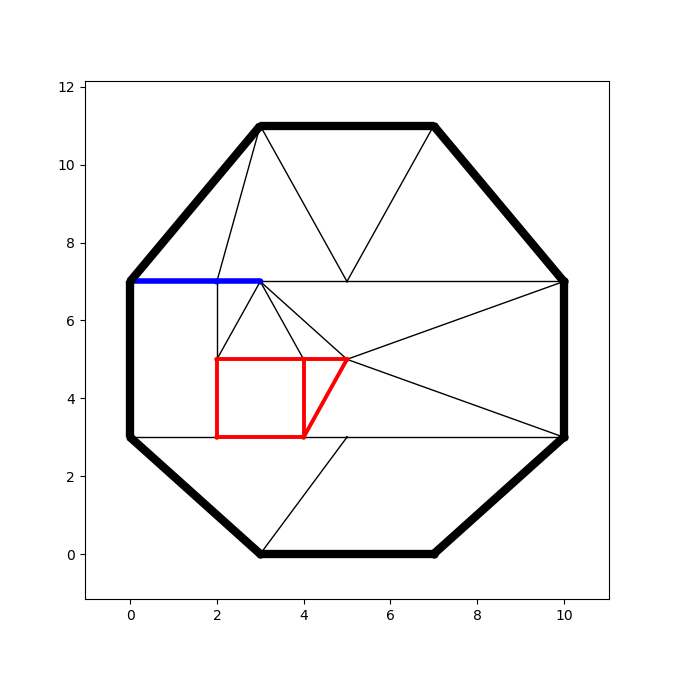
\includegraphics[width=1\textwidth]{images/Figure_6.png}
        \caption{$dt=0.1$}
        \label{fig:prob1_6_2}
    \end{minipage}
\end{figure}


\begin{figure}[H]
    \centering
    \begin{minipage}{.4\linewidth}
        \centering
        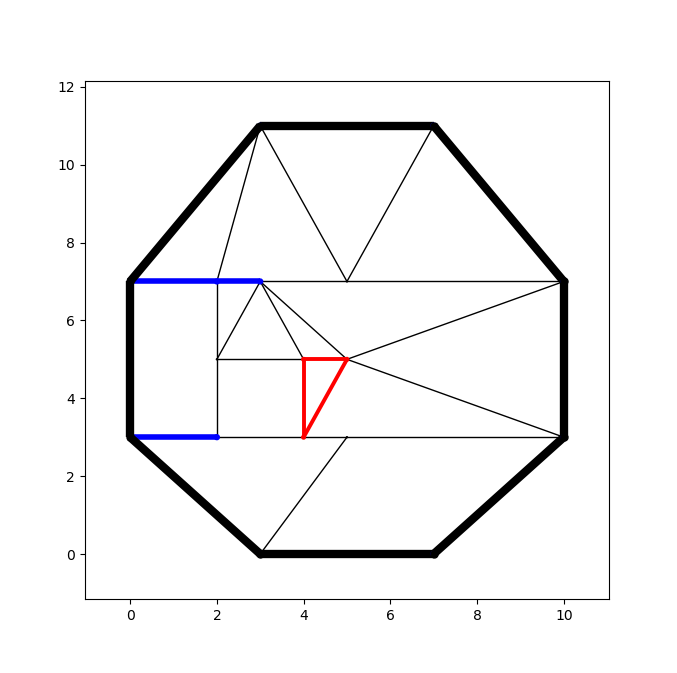
\includegraphics[width=1\textwidth]{images/Figure_7.png}
        \caption{$dt=0.1$}
        \label{fig:prob1_6_2}
    \end{minipage}%
    \begin{minipage}{.4\linewidth}
        \centering
        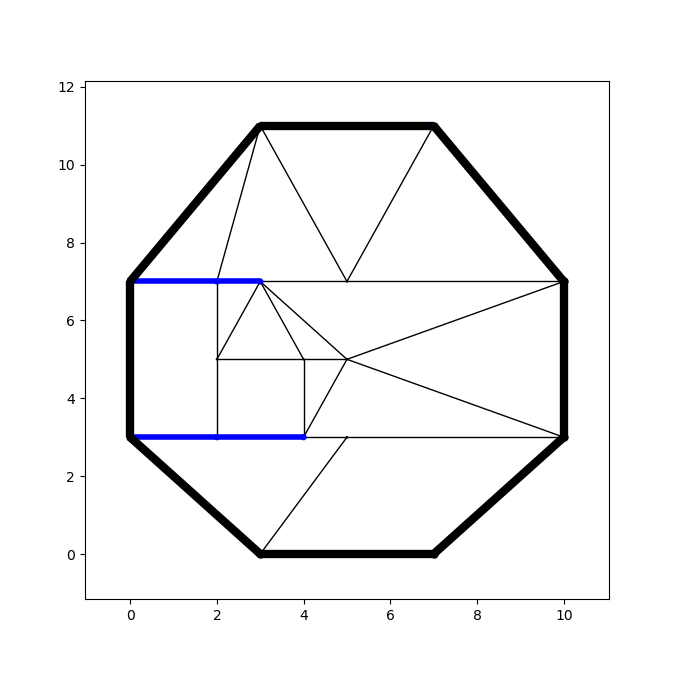
\includegraphics[width=1\textwidth]{images/Figure_8.png}
        \caption{$dt=0.1$}
        \label{fig:prob1_6_2}
    \end{minipage}
\end{figure}

In the figure () and figure (), we can see the dual graphs $S_0$ and $S_1$, respectively. Since, $S_1$ is a tree the complexity of this block is 1. Therefore, this block is universally accessible.

\begin{figure}[H]
    \centering
    \begin{minipage}{.4\linewidth}
        \centering
        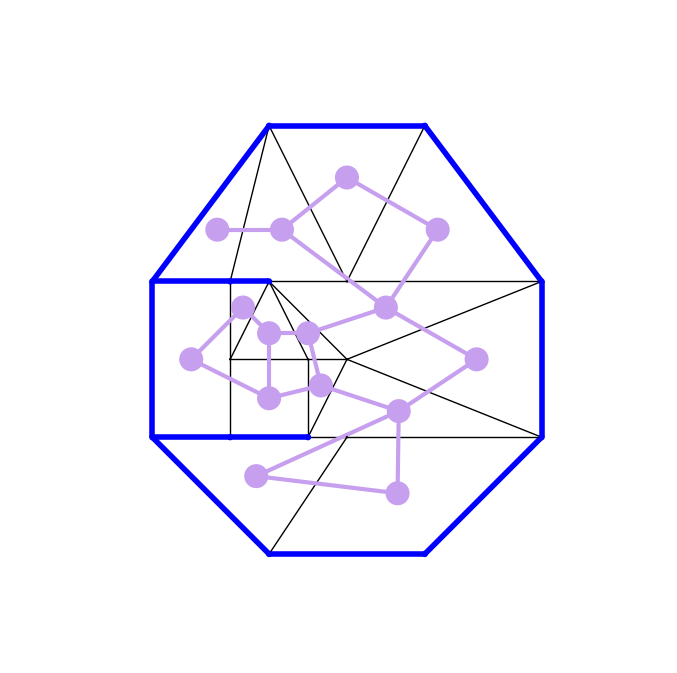
\includegraphics[width=1\textwidth]{images/Figure_9.png}
        \caption{$dt=0.1$}
        \label{fig:prob1_6_2}
    \end{minipage}%
    \begin{minipage}{.4\linewidth}
        \centering
        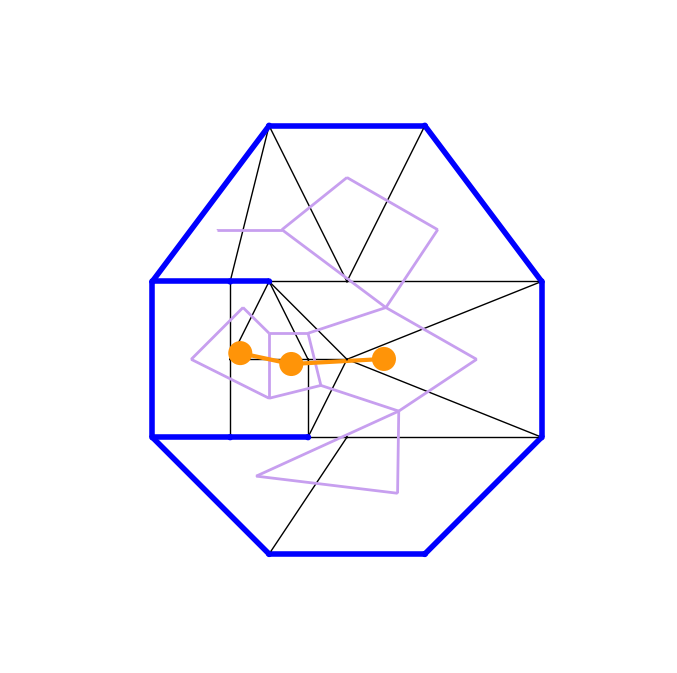
\includegraphics[width=1\textwidth]{images/Figure_11.png}
        \caption{$dt=0.1$}
        \label{fig:prob1_6_2}
    \end{minipage}
\end{figure}

Following, two solutions obtained using the statistical optimization approach is showing in the figure () and figure (). One solution path have around of 7.82 meters of new streets, while the other solution has around of 6.83 meters of new roads. Since, the optimal path solution computed with the strict optimization (piecewise) strategic, have a length of 7 meters of new streets, see fig(). This shows that the solution constructed using the strict optimization (piecewise) is not always the globally optimum.

\begin{figure}[H]
    \centering
    \begin{minipage}{.45\linewidth}
        \centering
        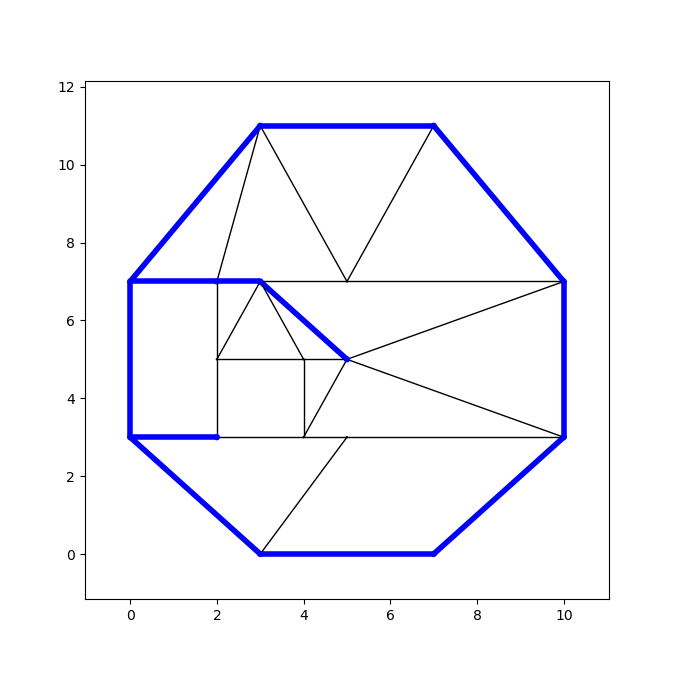
\includegraphics[width=1\textwidth]{images/Figure_14.png}
        \caption{$dt=0.1$}
        \label{fig:prob1_6_2}
    \end{minipage}%
    \begin{minipage}{.45\linewidth}
        \centering
        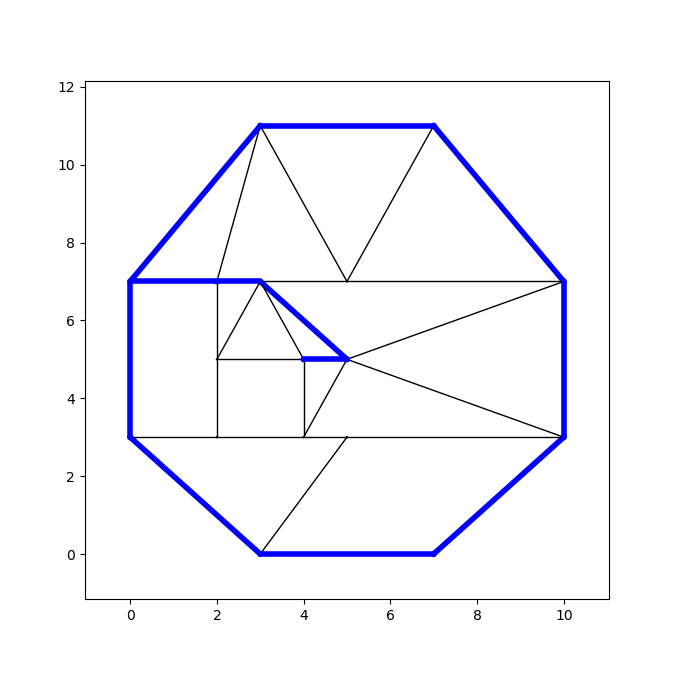
\includegraphics[width=1\textwidth]{images/Figure_13.png}
        \caption{$dt=0.1$}
        \label{fig:prob1_6_2}
    \end{minipage}
\end{figure}


\subsection{Implementation on Sector of the \emph{Ciudad de Dios} neighborhood}

The example of real life was developed in a section of \emph{Ciudad de Dios}, in Guayaquil. This sector has about 377 parcels of which, 281 are interior parcels, see fig().

\begin{figure}[H]
    \centering
    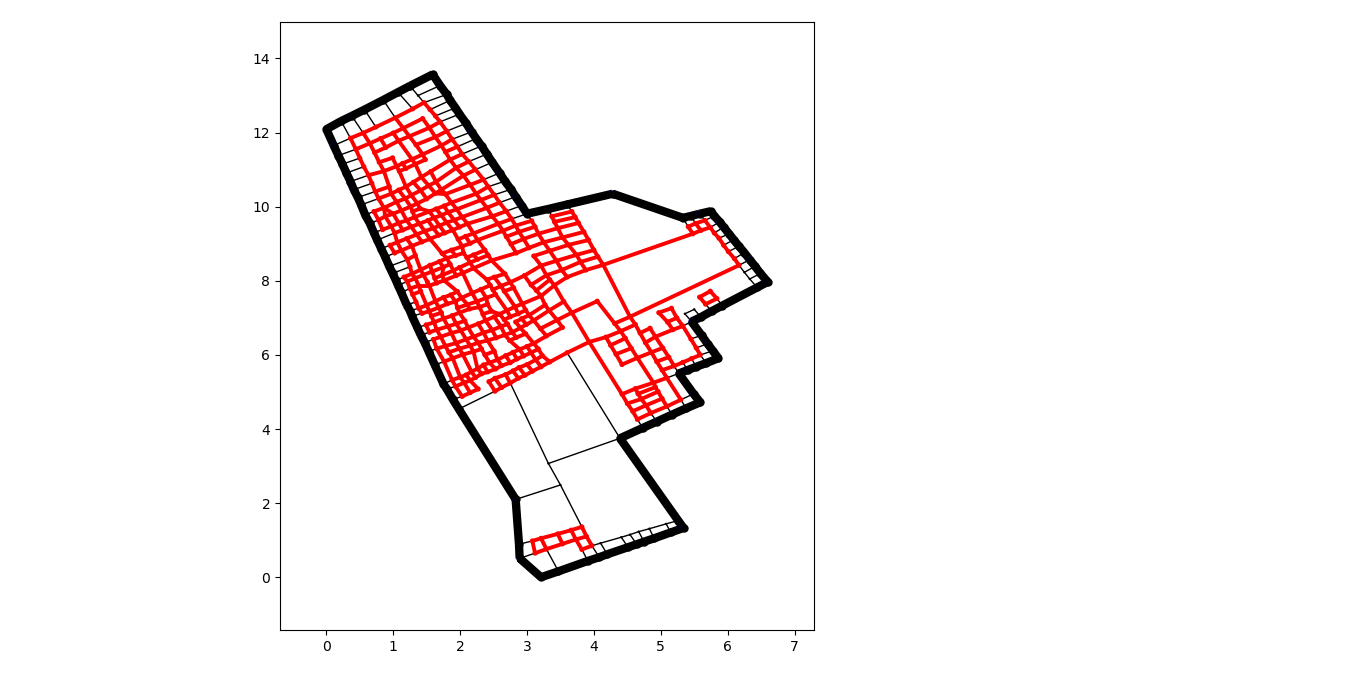
\includegraphics[width=0.6\textwidth]{images/parcels}
    \caption{Caption}
    \label{fig:my_label}
\end{figure}

The result of executing the statistical optimization give us a block that is universally accessible. Therefore, it is topological equivalent to a planned neighborhood, see fig().

\begin{figure}[H]
    \centering
    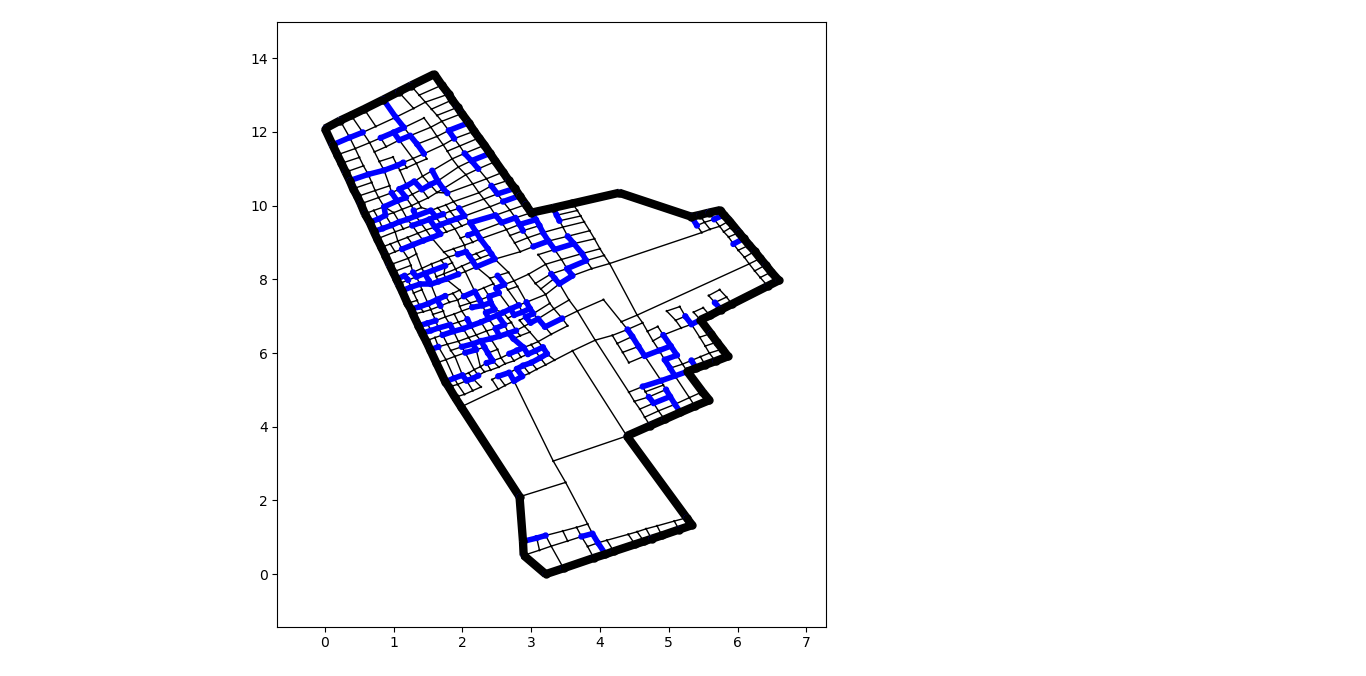
\includegraphics[width=0.6\textwidth]{images/parcels_2}
    \caption{Caption}
    \label{fig:my_label}
\end{figure}


\section{Conclusions}
Studying the neighborhoods and cities through topological tools and graph theory allowed to generate a characterization of the slums with respect to planned neighborhoods. It was found that the planned neighborhoods are universally accessible, i. e., all their parcels are connected to the network access system. While slums are not universally accessible. This characteristic can be determine using a topological tool called weak dual graphs; because it was found that a block is universally accessible, if and only if, his corresponding stage-two graph $S_2$ is a tree.\\ 

This results allow us to develop an algorithmic solution of the re-blocking problem with optimal cost\cite{bre}. Since executing an optimization algorithm could be a high time consuming process, an statistical optimization algorithm was proposed. The advantage of this approach is that we can add more information about the re-blocking problem and instead of having the global optimal solution we could have a more suitable solution to be implemented in the slum.\\

Given the characteristics of most of the slums in Ecuador, it could be said that implementing this mathematical approach in Ecuador could improve the situation of many cities in this country.


%%%%%%% Bibliografía %%%%%%%%
\bibliographystyle{bst/IEEEtran} 
\addcontentsline{toc}{section}{References}  
\bibliography{bib/IEEEreferences} 
%%%%%%% Bibliografía %%%%%%%%    

\appendix  
\clearpage % o \cleardoublepage
\addappheadtotoc 
\appendixpage

\section{Code in Python}
\begin{lstlisting}[language=Python]


# clean up and probability functions
def WeightedPick(d):
    """picks an item out of the dictionary d, with probability proportional to
    the value of that item.  e.g. in {a:1, b:0.6, c:0.4} selects and returns
    "a" 5/10 times, "b" 3/10 times and "c" 2/10 times. """

    r = random.uniform(0, sum(d.values()))
    s = 0.0
    for k, w in d.items():
        s += w
        if r < s:
            return k
    return k
    
    
def shorten_path(ptup):
    """ all the paths found in my pathfinding algorithm start at the fake
    road side, and go towards the interior of the parcel.  This method drops
    nodes beginning at the fake road node, until the first and only the
    first node is on a road.  This gets rid of paths that travel along a
    curb before ending."""

    while ptup[1].road is True and len(ptup) > 2:
        ptup.pop(0)
    return ptup


def segment_near_path(myG, segment, pathlist, threshold):
    """returns True if the segment is within (geometric) distance threshold
    of all the segments contained in path is stored as a list of nodes that
    strung together make up a path.
    """
    # assert isinstance(segment, mg.MyEdge)

    # pathlist = ptup_to_mypath(path)

    for p in pathlist:
        sq_distance = segment_distance_sq(p, segment)
        if sq_distance < threshold**2:
            return True

    return False
    
def shortest_path_p2p(myA, p1, p2):
    """finds the shortest path along fencelines from a given interior parcel
    p1 to another parcel p2"""

    __add_fake_edges(myA, p1, roads_only=True)
    __add_fake_edges(myA, p2, roads_only=True)

    path = nx.shortest_path(myA.G, p1.centroid, p2.centroid, "weight")
    length = nx.shortest_path_length(myA.G, p1.centroid, p2.centroid, "weight")

    myA.G.remove_node(p1.centroid)
    myA.G.remove_node(p2.centroid)

    return path[1:-1], length

def find_short_paths(myA, parcel, barriers=True, shortest_only=False):
    """ finds short paths from an interior parcel,
    returns them and stores in parcel.paths  """

    rb = [n for n in parcel.nodes+parcel.edges if n.road]
    if len(rb) > 0:
        raise AssertionError("parcel %s is on a road") % (str(parcel))

    if barriers:
        barrier_edges = [e for e in myA.myedges() if e.barrier]
        if len(barrier_edges) > 0:
            myA.remove_myedges_from(barrier_edges)
        else:
            print("no barriers found. Did you expect them?")
        # myA.plot_roads(title = "myA no barriers")

    interior, road = shortest_path_setup(myA, parcel)

    shortest_path = nx.shortest_path(myA.G, road, interior, "weight")
    if shortest_only is False:
        shortest_path_segments = len(shortest_path)
        shortest_path_distance = path_length(shortest_path[1:-1])
        all_simple = [shorten_path(p[1:-1]) for p in nx.all_simple_paths(myA.G,
                      road, interior, cutoff=shortest_path_segments + 2)]
        paths = dict((tuple(p), path_length(p)) for p in all_simple
                     if path_length(p) < shortest_path_distance*2)
    if shortest_only is True:
        p = shorten_path(shortest_path[1:-1])
        paths = {tuple(p): path_length(p)}

    myA.G.remove_node(road)
    myA.G.remove_node(interior)
    if barriers:
        for e in barrier_edges:
            myA.add_edge(e)

    parcel.paths = paths

    return paths

def find_short_paths_all_parcels(myA, flist=None, full_path=None,
                                 barriers=True, quiet=False,
                                 shortest_only=False):
    """ finds the short paths for all parcels, stored in parcel.paths
    default assumes we are calculating from the outside in.  If we submit an
    flist, find the parcels only for those faces, and (for now) recaluclate
    paths for all of those faces.
    """
    all_paths = {}
    counter = 0

    if flist is None:
        flist = myA.interior_parcels

    for parcel in flist:
        # if paths have already been defined for this parcel
        # (full path should exist too)
        if parcel.paths:

            if full_path is None:
                raise AssertionError("comparison path is None "
                                     "but parcel has paths")

            rb = [n for n in parcel.nodes+parcel.edges if n.road]
            if len(rb) > 0:
                raise AssertionError("parcel %s is on a road" % (parcel))

            needs_update = False
            for pathitem in parcel.paths.items():
                    path = pathitem[0]
                    mypath = ptup_to_mypath(myA, path)
                    path_length = pathitem[1]
                    for e in full_path:
                        if segment_near_path(myA, e, mypath, path_length):
                            needs_update = True
                            # this code would be faster if I could break to
                            # next parcel if update turned true.
                            break

            if needs_update is True:
                paths = find_short_paths(myA, parcel, barriers=barriers,
                                         shortest_only=shortest_only)
                counter += 1
                all_paths.update(paths)
            elif needs_update is False:
                paths = parcel.paths
                all_paths.update(paths)
        # if paths have not been defined for this parcel
        else:
            paths = find_short_paths(myA, parcel, barriers=barriers,
                                     shortest_only=shortest_only)
            counter += 1
            all_paths.update(paths)
    if quiet is False:
        pass
        # print("Shortest paths found for {} parcels".format(counter))

    return all_paths


def build_path(myG, start, finish):
    ptup = nx.shortest_path(myG.G, start, finish, weight="weight")

    ptup = shorten_path(ptup)
    ptup.reverse()
    ptup = shorten_path(ptup)

    mypath = ptup_to_mypath(myG, ptup)

    for e in mypath:
        myG.add_road_segment(e)

    return ptup, mypath


def choose_path(myG, paths, alpha, strict_greedy=False):

    """ chooses the path segment, choosing paths of shorter
    length more frequently  """

    if strict_greedy is False:
        inv_weight = dict((k, 1.0/(paths[k]**alpha)) for k in paths)
        target_path = WeightedPick(inv_weight)
    if strict_greedy is True:
        target_path = min(paths, key=paths.get)

    mypath = ptup_to_mypath(myG, target_path)

    return target_path, mypath
    
\end{lstlisting}

\newpage
\section{Euler's Figures from ‘Solutio problematis ad geometriam situs pertinentis.’}
\begin{figure}[H]
    \centering
    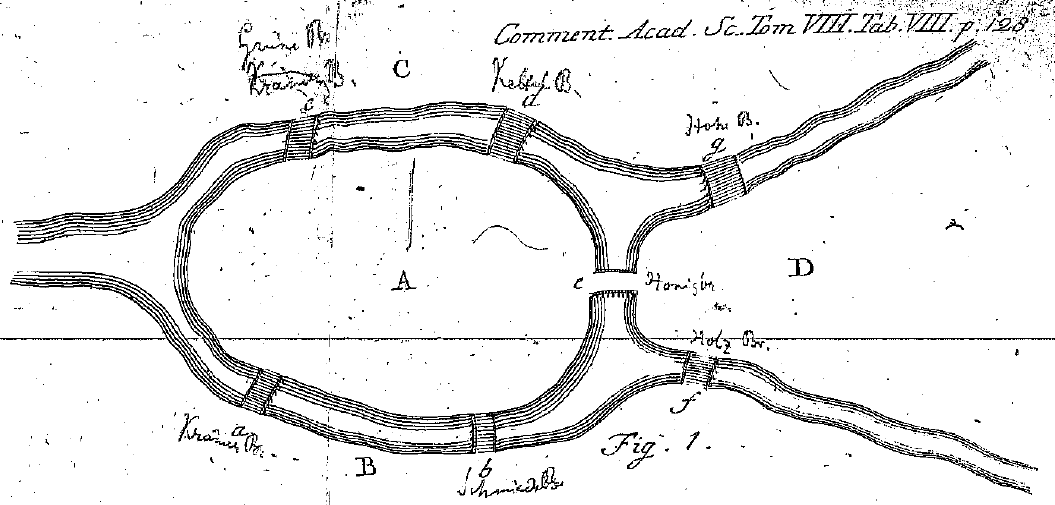
\includegraphics[width=0.75\textwidth]{images/Solutio_problematis_ad_geometriam_situs_pertinentis_Fig_1.png} 
    \caption{Caption}
    \label{fig:my_label}
\end{figure}

\begin{figure}[H]
    \centering
    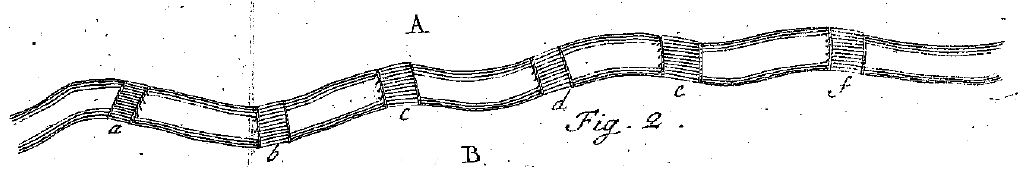
\includegraphics[width=0.75\textwidth]{images/Solutio_problematis_ad_geometriam_situs_pertinentis_Fig_2.png} 
    \caption{Caption}
    \label{fig:my_label}
\end{figure}

 
\begin{figure}[H]
    \centering
    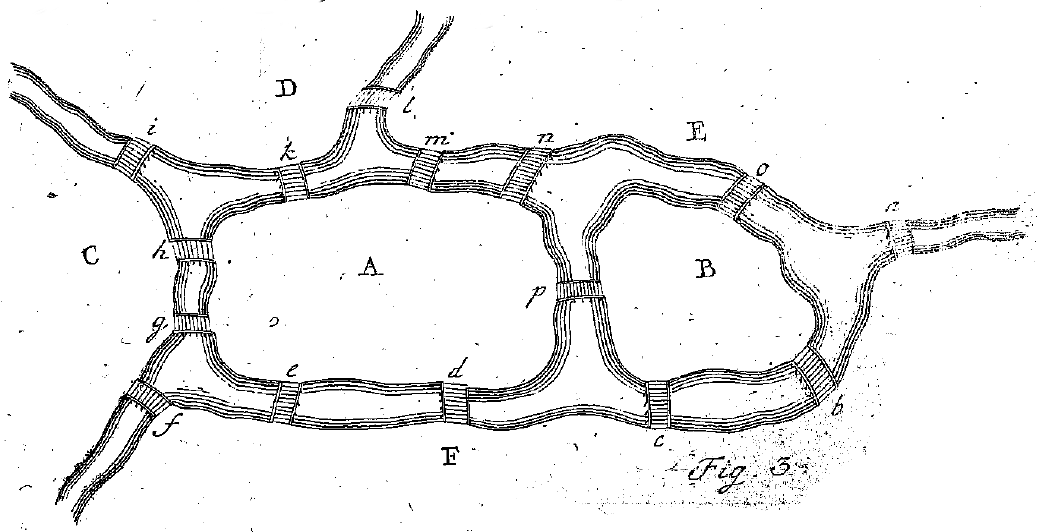
\includegraphics[width=0.75\textwidth]{images/Solutio_problematis_ad_geometriam_situs_pertinentis_Fig_3.png} 
    \caption{Caption}
    \label{fig:my_label}
\end{figure}


\end{document}
